\FloatBarrier
\section{OpenMP Experiments}
\label{sec:OMPExperiments}

Section~\ref{sec:OMP} describes the possibility of OpenMP-assisted multi-threading in most of the data-oblivious sorting algorithms used in this thesis. In that section, we also describe how each individual algorithm has been modified in order to support classical multi-threading.

In this set of experiments we extend our findings with experimental data showing the impacts of multi-threading.

Keep in mind that the \texttt{Intel i7-M620}, is a dual-core CPU using hyper-threading, which gives us two physical cores, able to run four simultaneous threads. This should give us an upper limit on the speed-up achieved to be four, but in practise this will be far from achievable. 

The setups of the algorithms are identical to those of Section~\ref{sec:Performance} and~\ref{sec:ShellsortExperiments}. Annealing Sort is not included, due to being highly serial.

\subsection{Running Time}

\begin{figure}
\center
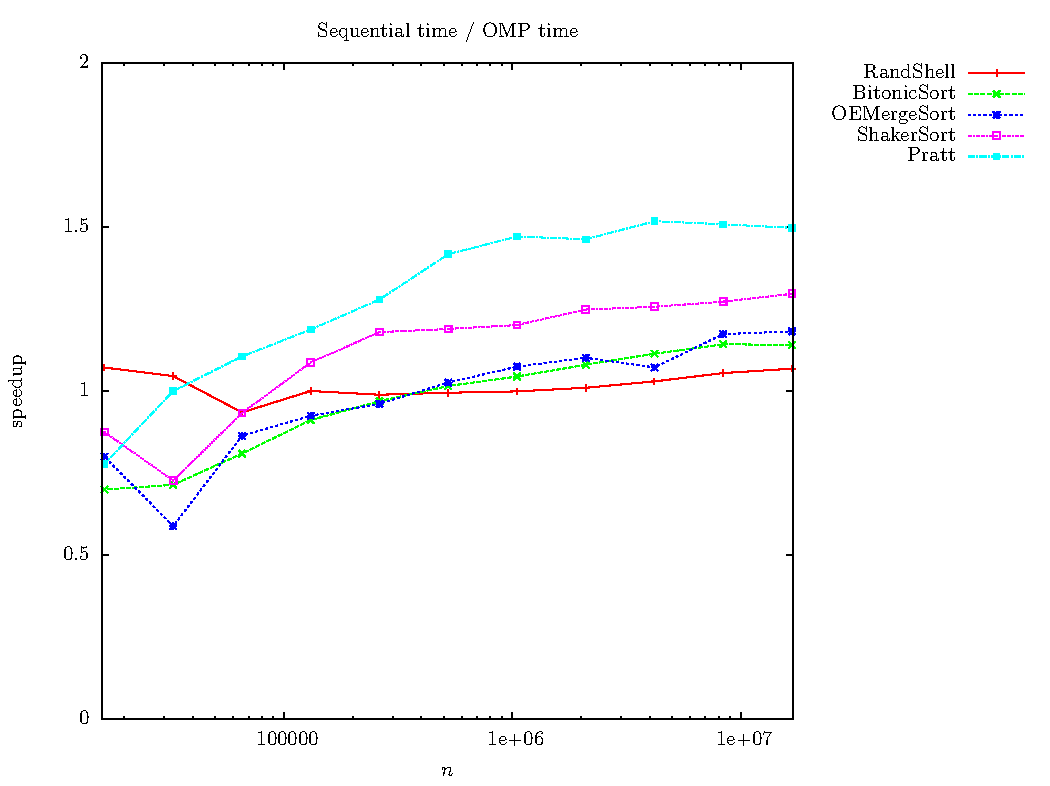
\includegraphics[width=\textwidth]{graphs/OMP/timediff.pdf}
\caption{Running Time improvement by OpenMP application}
\label{fig:OMP:timediff}
\end{figure}

Let us start by looking at the actual running time of the algorithms.
Figure~\ref{fig:OMP:timediff} shows the factor gained in execution speed when OpenMP is applied, as a measure of wall-clock time for each algorithm. The value for the largest input size is shown are collected in Table~\ref{tab:OMP:timedifffinal}.

\begin{table}[!h]
\begin{adjustwidth}{-.5in}{-.5in}
\centering
\begin{tabular}{|l|c|c|c|c|c|}
\hline
Algorithm & Randomized Shellsort & Bitonic Sort & Odd-Even Mergesort & Pratt & Shaker Sort \\ \hline
Factor    & 1.07                 & 1.14         & 1.18 & 1.50 & 1.29           \\ \hline
\end{tabular}
\caption{OpenMP gain for largest input size, $2^24$}
\label{tab:OMP:timedifffinal}
    \end{adjustwidth}
\end{table} 

Randomized Shellsort gets a small improvement from multi-threading, since some parts of the algorithm can be executed in parallel, though a great deal synchronization is required.

Both Bitonic Sort and Odd-Even Mergesort show a better application of multi-threading, and achieve a higher improvement in running time, due to the recursive calls adapting well to the task-based methodology of OpenMP.

Finally we see the two normal Shellsort variants both achieve a substantial  improvement in running time by using OpenMP. This great benefit of multi-threading in the simple Shellsort variants stems from the intrinsic separation of sub-sequences in the algorithms. Pratt's Shellsort impressively tops the chart by having many sub-sequences that divide evenly into the amount of threads, and handling these in a simpler manner than Shaker Sort.

These running times all show that we are far from even utilizing both cores fully, and even further from the 4-factor speedup that might be possible when fully utilizing hyper-threading. Let us further investigate why we are not anywhere near maximum utilization.

\subsection{Instructions, Cache Misses and Branch Mispredictions}

\begin{figure}
\center
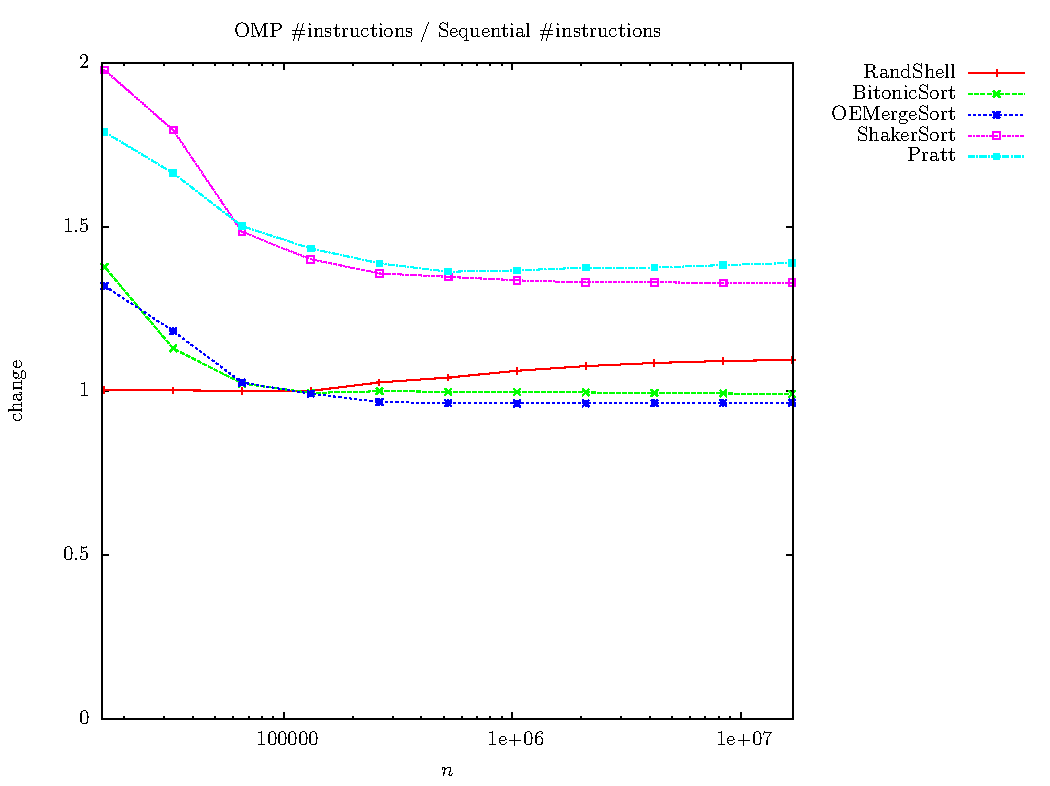
\includegraphics[width=\textwidth]{graphs/OMP/instrdiff.pdf}
\caption{Instruction degradation by OpenMP application}
\label{fig:OMP:instrdiff}
\end{figure}

\begin{figure}
\center
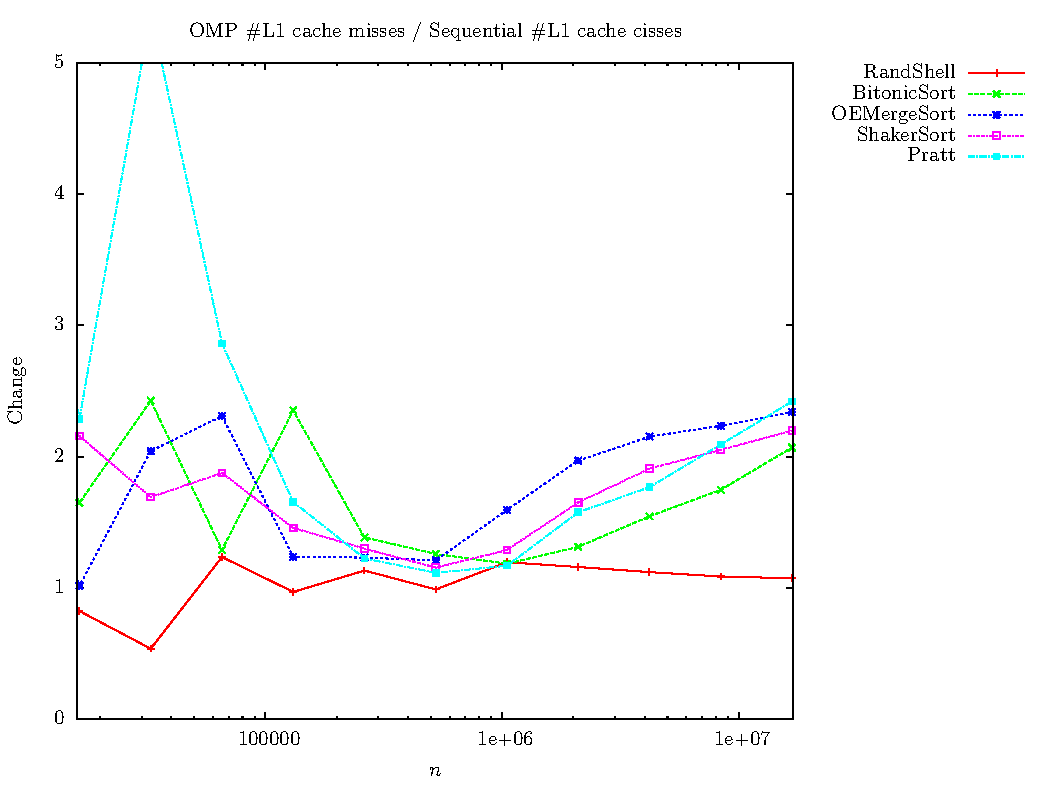
\includegraphics[width=\textwidth]{graphs/OMP/cachediff.pdf}
\caption{Cache degradation by OpenMP application}
\label{fig:OMP:cachediff}
\end{figure}

\begin{figure}
\center
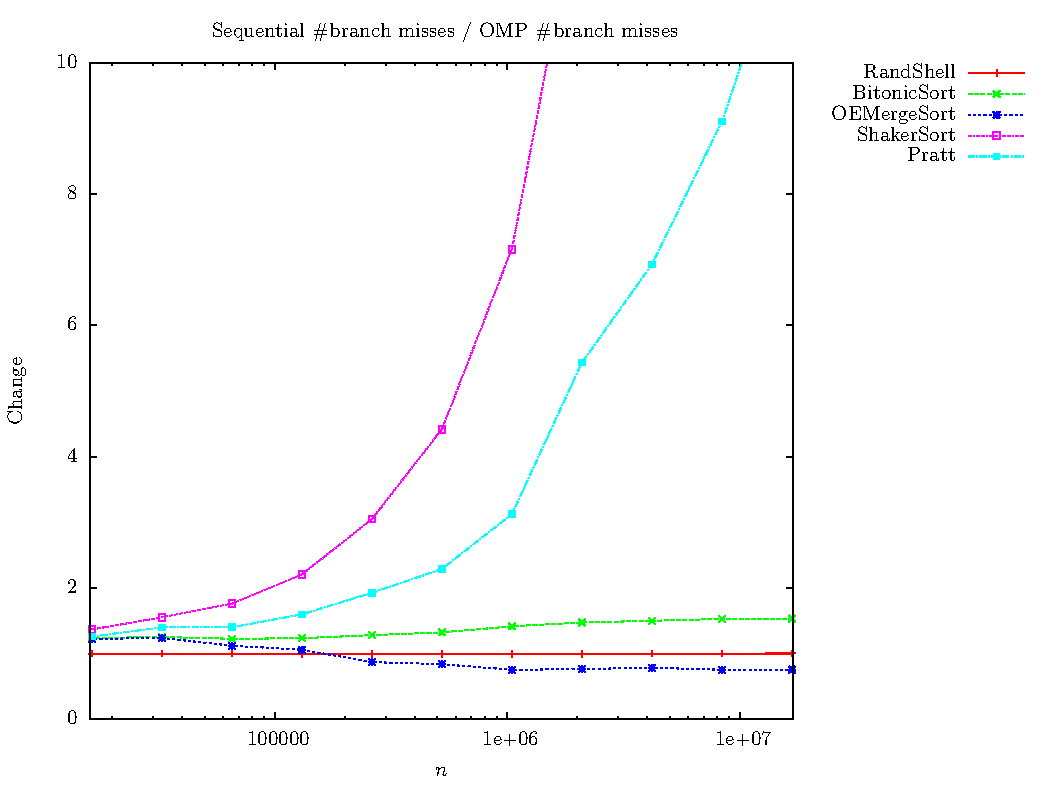
\includegraphics[width=\textwidth]{graphs/OMP/branchdiff.pdf}
\caption{Branch degradation by OpenMP application}
\label{fig:OMP:branchdiff}
\end{figure}

In order to explain the non-optimal utilization of CPU time, we must study the low-level hardware characteristics.

Instructions are a major factor in execution time, and each type of algorithm is affected differently when applying multi-threading.
Randomized Shellsort sees a slightly increased instruction count due to threading overhead, but the high baseline instruction count keeps this impact low. 
Bitonic Sort and Odd-Even Mergesort both see a minor effect from multi-threading, and there is even a reduction in instructions. This effect is strange, but is likely due to the low instruction overhead of OpenMP tasks, and some compiler magic
\footnote{Compilation is done using \texttt{Ofast}, which favours speed over executable size, which may have an adverse effect on instruction count.}.
Finally, we see Pratt's Shellsort and Shaker Sort having a high instruction overhead, due to complicated threading control, and a low baseline.

For the L1 cache misses, we see Randomized Shellsort having a small increase, due to a high baseline. The other algorithms show a moderate increase in L1 cache misses due to data sharing between the CPU cores.

In branch misses, we see almost no increase for Randomized Shellsort, due to a high baseline. Bitonic Sort increases slightly, due to thread synchronization, while Odd-Even Mergesort strangely decreases \footnote{
Explaining a decrease in branch mispredictions when applying multi-threading is difficult. Possible causes might be changes in the inlining strategy, or a collision in prediction counters when operating in single-threaded mode. Alternatively, having each recursive call separated to a single thread might prevent mispredictions across calls.
}. The two variants of Shellsort see major increase in branch mispredictions, due to having a great amount of logic applied in the scheduling of threads, and a low baseline.

\subsection{Experiment Conclusions}

This set of experiments shows that OpenMP is a viable strategy for improving the performance of data-oblivious sorting algorithms, though not nearly as effective as SIMD and CUDA. We also identify several performance issues keeping the OpenMP implementation from achieving the maximum possible performance gain.